\documentclass[11pt, a4paper]{scrartcl}

\usepackage{vorschule}
\usepackage[
    typ=ab,
    fach=Mathematik,
    lerngruppe={6b},
    nummer=15,
    module={Symbole,Papiertypen},
]{schule}

\usepackage[
	kuerzel=Ngb,
	reihe={Mit Brüchen und Dezimalzahlen rechnen},
	version={2019-03-14},
]{ngbschule}

\author{J. Neugebauer}
\title{Dezimalzahlen multiplizieren}
\date{\Heute}

\setzeAufgabentemplate{ngbnormal}


\begin{document}
	\ReiheTitel
	
	\begin{aufgabe}
		Forme die Dezimalzahlen in Brüche um, rechne aus und schreibe das Ergebnis wieder als Dezimalzahl.
		
		\begin{enumeratea}
			\item $0,4\cdot 0,03 = \frac{4}{10}\cdot \frac{3}{100} = $\linievoll
			\item $0,04\cdot 0,3 = $\linievoll
			\item $0,5\cdot 0,005 = $\linievoll
			\item $1,2\cdot 3,4 = $\linievoll
			\item $12\cdot 0,34 = $\linievoll
		\end{enumeratea}
	\end{aufgabe}

	\begin{aufgabe}
		Betrachte die Rechnungen und Ergebnisse aus Aufgabe 1. Kannst du Regelmäßigkeiten erkennen?\smallskip
		
		Formuliere eine Regel zur \emph{Multiplikation von Dezimalzahlen}, \dashuline{ohne sie in Brüche umzuformen}.\smallskip
		
		\feldLin[1cm]{4}
		
		\hinweis{Achte auf die \emph{Anzahl der Nachkommastellen} der Zahlen.}
	\end{aufgabe}

	\begin{aufgabe}
		Notiere drei weitere Beispielrechnungen.
		
		\feldLin[1cm]{3}
	\end{aufgabe}
	
	\begin{aufgabe}
		\begin{wrapfigure}{r}{2cm}
			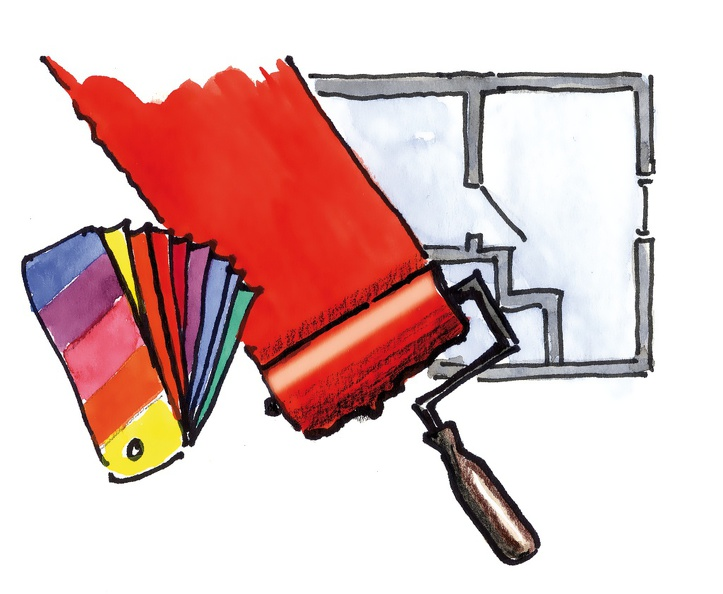
\includegraphics[width=2cm]{6.15-Abb_Renovieren.jpg}
		\end{wrapfigure}
		Hannes soll in seinem Kinderzimmer einen neuen Teppich bekommen. Er hat ausgemessen, dass sein Zimmer \unit[$4,5$]{m} breit und \unit[$3,6$]{m} lang ist. Ein Quadratmeter des Teppichs, den er sich ausgesucht hat, kostet \unit[$4,99$]{\euro}.\medskip
		
		Wie viel kostet der neue Teppich insgesamt?\medskip
		
		\feldKar{6}
	\end{aufgabe}
\end{document}